\chapter{Previsão}
\label{cap:prev}

\section{O melhor previsor}
Para erro quadrático, o melhor previsor de $y_{T+h}$ dado o passado é a esperança condicional $\E(y_{T+h}\mid y_T,y_{T-1},\dots)$ (capítulo~\ref{cap:ec}). Num AR(1) com média $\mu$:
\[
\hat y_{T+h}=\mu+\phi^h(y_T-\mu),\qquad \Var(e_{T+h})=\sigma^2\,\frac{1-\phi^{2h}}{1-\phi^2}.
\]
\begin{intuicao}
Quanto mais longe o horizonte, mais a previsão se aproxima da média de longo prazo, e mais a incerteza se aproxima da variância incondicional $\gamma_0=\sigma^2/(1-\phi^2)$. Para $h$ grande, o modelo não sabe mais do que a média.
\end{intuicao}

\begin{center}
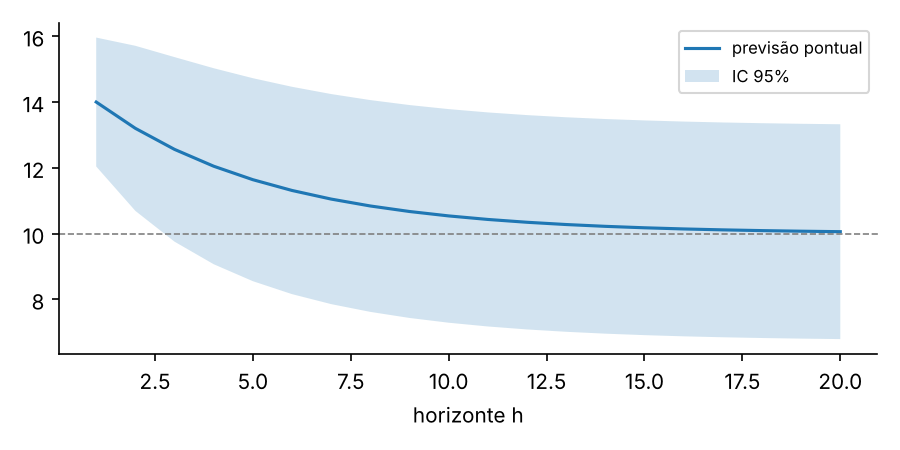
\includegraphics[width=0.75\textwidth]{fig/previsao_ar1.png}\\
\small AR(1) com $\mu=10$, $\phi=0{,}8$, $\sigma=1$ e último desvio $y_T-\mu=5$. A previsão decai para a média e o intervalo alarga e estabiliza.
\end{center}

\begin{simulacao}[{Conferido por simulação: cobertura do intervalo}]
Simulei 4000 séries AR(1) com $\phi=0{,}8$, previ $h=3$ passos à frente e construí o intervalo de 95\%. A cobertura empírica foi $95{,}0\%$. A variância teórica do erro para $h=3$ é $(1-0{,}8^6)/(1-0{,}64)=2{,}0496$, confirmada.
\end{simulacao}

\section{Passeio aleatório e ARIMA}
Num passeio aleatório, $\hat y_{T+h}=y_T$ (previsão ``ingênua'') e $\Var(e_{T+h})=h\sigma^2$. O intervalo cresce sem parar, o que reflete a natureza de choques permanentes. Modelos ARIMA com $d\ge1$ têm essa mesma propriedade, o que é muito diferente de um modelo estacionário.

\begin{atencao}[{Armadilha: intervalos otimistas}]
Os intervalos clássicos tratam os parâmetros estimados como verdadeiros e supõem que o modelo está certo. Com amostras curtas ou escolha de modelo feita com os mesmos dados, a cobertura real costuma ser menor do que a nominal. Em previsão séria, avalie a cobertura fora da amostra.
\end{atencao}

\section{Como avaliar previsões}
\begin{itemize}[leftmargin=1.4em]
\item \textbf{Fora da amostra, sempre.} O ajuste dentro da amostra premia modelos complicados.
\item \textbf{Origem móvel (rolling origin)}: estime até $t$, preveja $t+1,\dots,t+h$, avance a origem e repita.
\item \textbf{Métricas}: MAE e RMSE (mesma unidade da série); MAPE é intuitivo, mas explode se há valores próximos de zero e pune erros positivos e negativos de forma assimétrica; MASE compara com o previsor ingênuo e é comparável entre séries.
\item \textbf{Sempre inclua um \emph{benchmark}}: ingênuo (último valor) ou sazonal ingênuo. Um modelo que não bate o ingênuo não serve.
\end{itemize}

\begin{exercicio}
AR(1) com $\mu=0$, $\phi=0{,}8$, $\sigma^2=1$ e último valor $y_T=5$. Dê a previsão para $h=3$ e o intervalo de 95\%.
\end{exercicio}
\sol{Previsão: $0{,}8^3\times5=0{,}512\times5=2{,}56$. Variância do erro: $2{,}0496$, desvio $1{,}4317$. Intervalo: $2{,}56\pm1{,}96\times1{,}4317=2{,}56\pm2{,}806$, isto é, $[-0{,}25;\,5{,}37]$.}

\begin{exercicio}
Um passeio aleatório tem $\sigma=2$. Qual é o desvio-padrão do erro de previsão a 9 passos?
\end{exercicio}
\sol{$\sqrt{h}\,\sigma=\sqrt9\times2=6$.}
